LIME (Local Interpretable Model-Agnostic Explanations) -- метод, показывающий вклад признаков в отдельное предсказание, работающий с любой моделью.
% нужен ли перевод

\subsubsection{Идея}
Результаты некоторых моделей легко интерпретировать. Например, в линейной регрессии можно посмотреть на веса. Они показывают, насколько изменится предсказание при изменении признаков. Так для каждого конкретного предсказания можно понять, почему модель выдала именно такой результат -- виден непосредственный вклад каждого признака.

Но не все модели легко интерпретировать. Например, некоторые архитектуры нейронных сетей. Они зачастую значительно превосходят линейные модели, но при этом сама структура модели представляет собой <<черный ящик>> -- непонятно, как именно модель сформировала предсказание, какие признаки сильнее повлияли на решение нейронной сети.

Идея состоит в том, чтобы перенести свойство интерпретируемости простых моделей на более сложные. Мы можем обучить интерпретируемую модель по выборке, где ответами являются предсказания сложной модели. В процессе обучения модель анализирует зависимости непосредственно между признаками и предсказаниями сложной модели. Тогда мы сможем интерпретировать результаты простой модели, которые являются аппроксимацией предсказаний сложной.\\[2mm]
\begin{minipage}{0.57\linewidth}
\indent Возникает проблема: сложная модель выявляет зависимости, которые, например, линейная модель может не уловить. Идея данного метода заключается в том, чтобы обучать более простую модель в некоторой окрестности исследуемого объекта, предполагая что на очень локальном уровне нет сложных зависимостей \cite{lime_dop}. Например, дифференцируемые функции можно линеаризовать в окрестности заданной точки -- можно использовать линейную модель на локальном уровне.
\end{minipage}
\hspace{5mm}
\begin{minipage}{0.35\linewidth}
	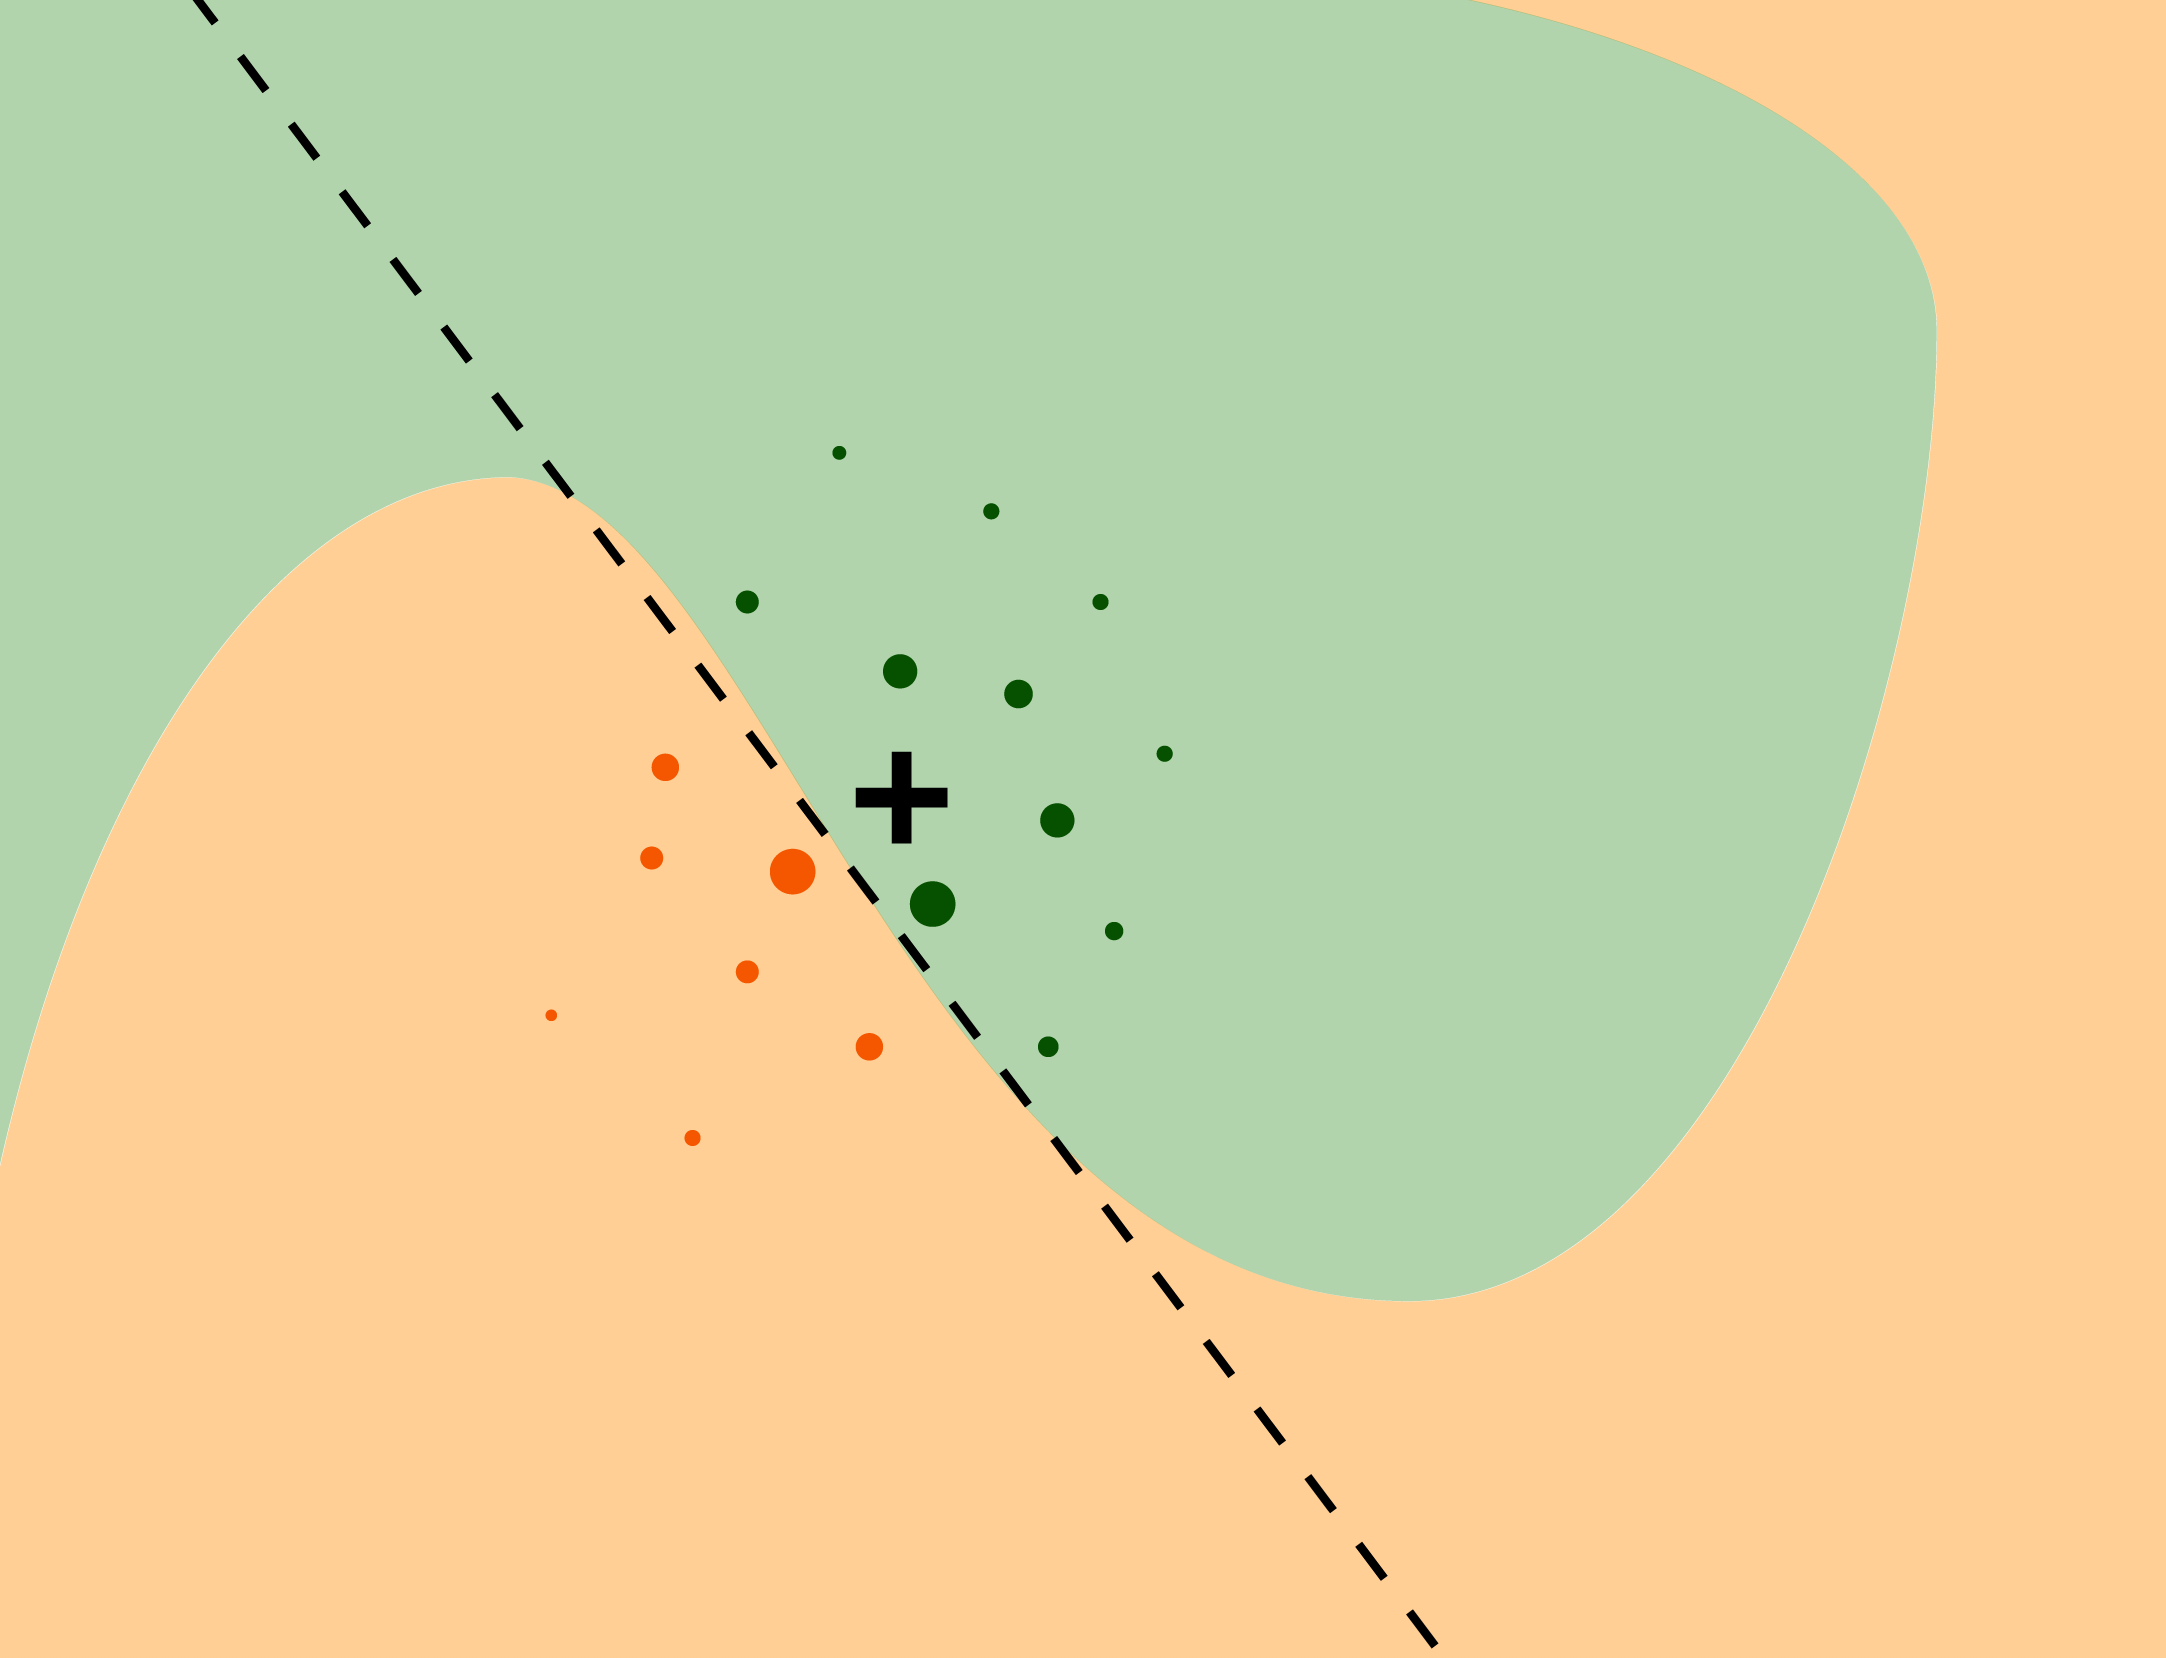
\includegraphics[width=6.5cm, height=5cm]{pics/lime4.png}
\end{minipage}

\underline{Пример LIME для табличных данных} \cite{limegit}
\vspace{-3mm}

\begin{figure}[h]
	\centering{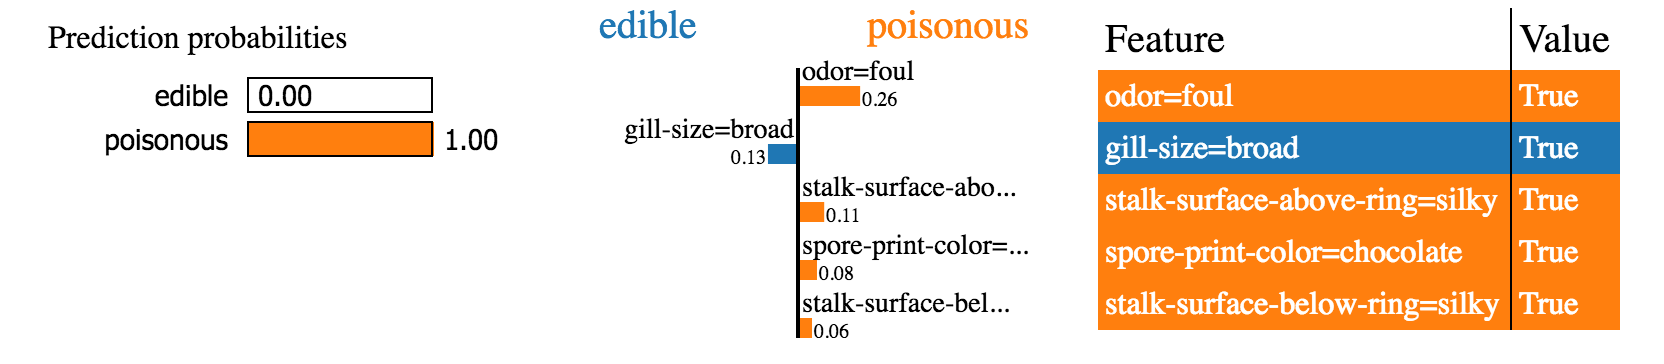
\includegraphics[width=\linewidth]{pics/lime1.png}}
\end{figure}

В данном случае решалась задача бинарной классификации. LIME вывел пять самых значимых признаков и показал, каким образом они повлияли на предсказание. Обученная модель показала, что исследуемый объект принадлежит к классу <<poisonous>>. И по анализу LIME понятно почему: только один признак из выведенных увеличил вероятность принадлежности объекта к классу <<edible>> и только на $0.13$. В то же время оставшиеся четыре признака повлияли на вероятность объекта быть <<poisonous>>, причем суммарно увеличив вероятность на $0.51$. Данная интерпретация позволяет понять, адекватна ли модель, которую мы получили, действительно ли релевантные признаки оказались значимыми.

\underline{Пример LIME для текстов} \cite{limegit}
\vspace{-3mm}

\begin{figure}[h]
	\centering{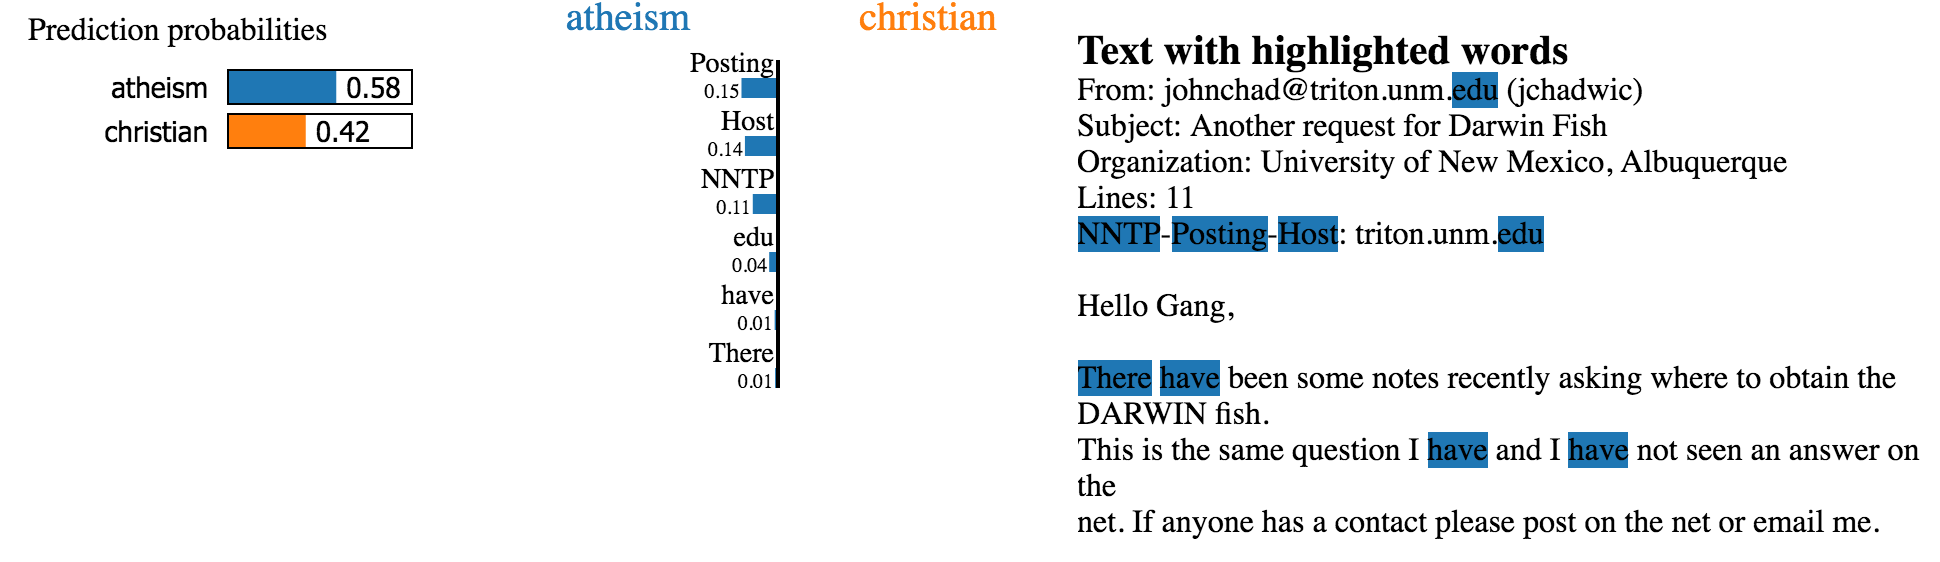
\includegraphics[width=\linewidth]{pics/lime2.png}}
\end{figure}

Вновь решалась задача бинарной классификации: определить, к какой теме (христианство/атеизм) относится документ. LIME выделил отдельные слова, которые, по его <<мнению>>, оказались наиболее важны для предсказания. Можно заметить, что слово <<Posting>> оказалось довольно-таки значимым, поскольку увеличило вероятность принадлежности текста к тематике атеизма на 0.15. Однако это несколько контринтуитивно, поскольку <<posting>> может относиться одинаково вероятно к обоим темам. Мы выявили недостаток в модели, к результатам ее работы стоит относиться аккуратно.

\underline{Пример LIME для картинок} \cite{lime_dop}
\vspace{-3mm}

\begin{figure}[h]
	\centering{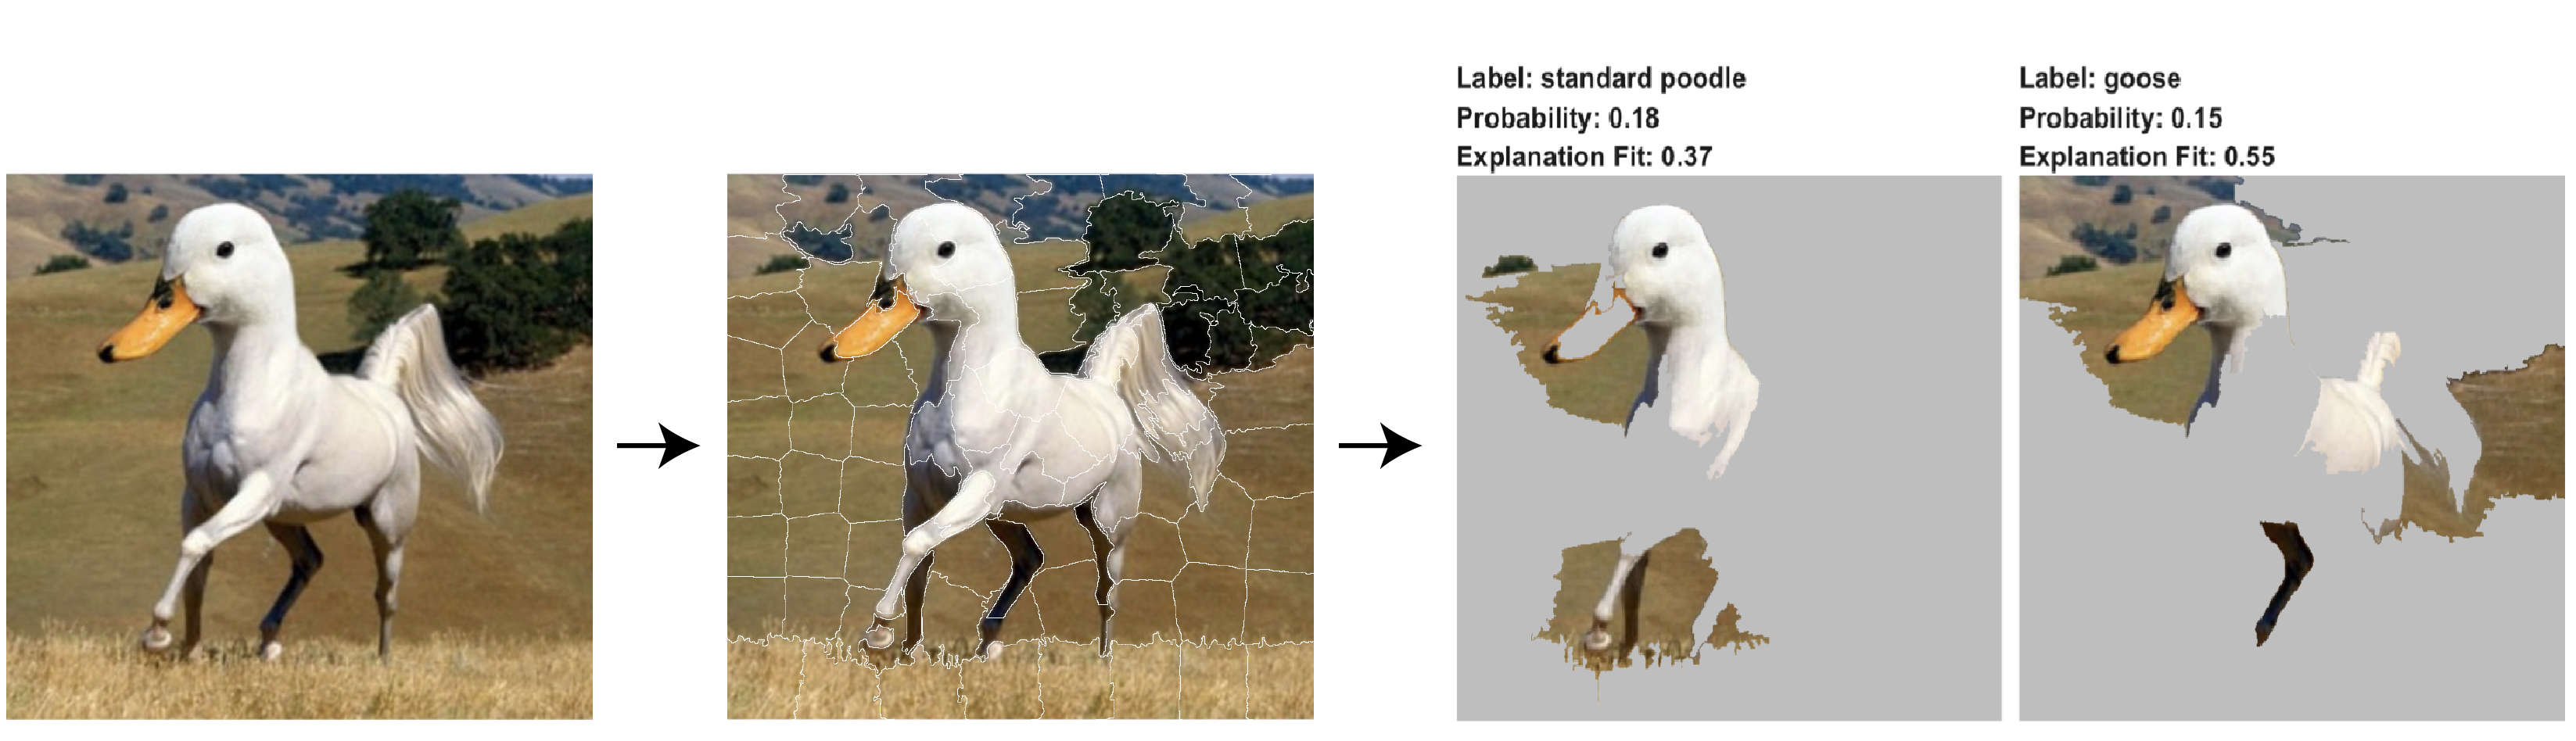
\includegraphics[width=\linewidth]{pics/lime3.png}}
\end{figure}

Интерпретация картинок с LIME наиболее понятная и интересная. Изображение было разбито на несколько частей (супер-пиксели). И далее алгоритм выбрал наиболее важные для получения того или иного ответа. На второй картинке LIME корректно выбрал фрагменты гуся, которые модель смогла распознать. Но на первой картинке модель ошиблась и выявила пуделя.